\section{Massimi e minimi}
\subsection{Massimo e minimo intervalli}
\begin{definition}[Massimo]
Dato un insieme A tale che: \\$A \subseteq \mathbb{R}, \: A \neq \O, \: m \in \mathbb{R}$ m si dice \textbf{massimo} di A se $m \geq a \: \forall \: a \in A$ e $m \in A$
\end{definition}
\begin{definition}[Minimo]
Dato un insieme A tale che: \\$A \subseteq \mathbb{R}, \: A \neq \O, \: m \in \mathbb{R}$ m si dice \textbf{minimo} di A se $m \leq a \: \forall \: a \in A$ e $m \in A$
\end{definition}
\begin{example}
    Esempi massini e minimi intervalli:
    \begin{itemize}
        \item Dato $A = [0,1]$ il max(A) = 1 e il suo min(A) = 0
        \item Dato $B = [0, 1)$ il min(B) = 0 mentre B non ha massimo.
    \end{itemize}
\end{example}

\begin{wrapfigure}{r}{8cm}
    \vspace{10pt}
    \centering
    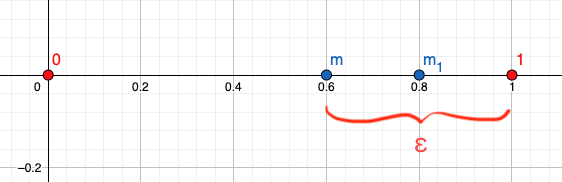
\includegraphics[width=7cm]{dimostrazione-massimo.png}
    \caption{Segmento B}
\end{wrapfigure}
\begin{demostration}
Dimostriamo questo esempio:
\end{demostration}
Supponiamo per assurdo che $m \in \mathbb{R}$ sia il max di B, con ovviamente $m \in B$. Se tale condizione è vera $m < 1$ perché 1 non è incluso nell'insieme B = [0, 1).\\ \\
Poniamo ora $\epsilon = 1 - m$, così facendo $\epsilon$ diventa la lunghezza dell'intervallo fra 1 ed m.\\ \\
Definiamo ora un $m_1 = m + \frac{\epsilon}{2}$. Creando questo valore $m_1$ vediamo che $m_1 \in B$ ma anche che $m < m_1$ che contrasta con la definizione di massimo di B che dovrebbe essere $m \geq b \: \forall \: b \in B$. Così dimostriamo la non esistenza di un valore massimo.

\subsection{Maggiorante e minorante intervalli}
\begin{definition}[Maggiorante]
$A \subseteq \mathbb{R}$, $A \neq \O$, $k \in \mathbb{R}$ si dice \textbf{maggiorante} di A se $k \geq a \: \: \forall \: \: a \in A$. L'insieme di tutti i maggioranti si indica con $M_A$.
\end{definition}
\begin{definition}[Minorante]
$A \subseteq \mathbb{R}$, $A \neq \O$, $k \in \mathbb{R}$ si dice \textbf{minorante} di A se $k \leq a \: \: \forall \: \: a \in A$. L'insieme di tutti i minoranti si indica con $m_A$.
\end{definition}
\begin{example}
A = [0,3] allora 3 è un maggiorante di A, quindi $3 \in M_A$. \\
Mentre $\frac{1}{4}$ non è un maggiorante, quindi $\frac{1}{4} \notin M_A$, perché $1 > A$ e $1 > \frac{1}{2}$.
\end{example}
\begin{observation}
    Se esiste un maggiorante di A allora ne esistono infiniti. Infatti se prendiamo un $k \in M_A$, m è un maggiorante di A $\forall \: \: m \geq k$.
    Questo discorso vale anche per i minoranti, infatti con $k \in m_A$, m è un minorante di A $\forall \: \: m \leq k$.
    \begin{example}
        Esempi per l'osservazione sopra:
        \begin{itemize}
            \item A = $\mathbb{R}$, A non ha maggioranti.
            \item A = [4, $+\infty$] non ha maggioranti ma ha minoranti.
        \end{itemize}
    \end{example}
\end{observation}

\subsection{Intervallo limitato}
\begin{definition}[Limitato superiormente]
    Dato un intervallo A, se $M_A \neq \O$ (insieme dei maggioranti) allora l'intervallo A si dice \textbf{limitato superiormente}
\end{definition}
\begin{definition}[Limitato inferiormente]
    Dato un intervallo A, se $m_A \neq \O$ (insieme dei minoranti) allora l'intervallo A si dice \textbf{limitato inferiormente}
\end{definition}
\begin{definition}[Limitato]
    $A \subset \mathbb{R}$, $A \neq \O$, se A è sia superiormente che inferiormente limitato allora A si dice semplicemente intervallo \textbf{limitato}.
\end{definition}
\begin{observation}
    A è limitato se e solo se $\exists \: \: h,k \in \mathbb{R}$ tale che $k \leq a \leq h \: \: \forall \: \: a \in A$
\end{observation}

\subsubsection{Estremi superiori ed inferiori}
\begin{theorem}[Estremo superiore]
    $A \subset \mathbb{R}$, $A \neq \O$ ed A è superiormente limitato, allora esiste il minimo dell'insieme dei maggioranti. Tale minimo si dice \textbf{estremo superiore} di A e si indica con sup(A).
\end{theorem}
\begin{theorem}[Estremo inferiore]
    $A \subset \mathbb{R}$, $A \neq \O$ ed A è inferiormente limitato, allora esiste il massimo dell'insieme dei minoranti. Tale massimo si dice \textbf{estremo inferiore} di A e si indica con inf(A).
\end{theorem}
\begin{example}
    Esempio estremi superiori ed inferiori:
    \begin{itemize}
        \item A = [0, 1) \hspace{.1cm} $M_A$ = [1, $+\infty$) e $m_A$ = ($-\infty$, 0] \hspace{.1cm} min($M_A$) = sup(A) = 1 \hspace{.2cm} max($m_A$) = inf(A) = 0
        \item B = [0, 1] \hspace{.1cm} $M_B$ = [1, $+\infty$) e $m_A$ = ($-\infty$, 0] \hspace{.1cm} min($M_B$) = sup(B) = 1 \hspace{.2cm} max($m_B$) = inf(B) = 0
    \end{itemize}
    \begin{observation}
        Se esiste max(A) allora max(A) = sup(A) e viceversa se esiste min(A) allora min(A) = inf(A)
    \end{observation}
\end{example}
\begin{note}
    Se A non è superiormente limitato scriviamo sup(A) = $-\infty$ e se non è inferiormente limitato inf(A) = $-\infty$.
\end{note}
\begin{observation}
    $A \neq \O$ e A è superiormente limitata, allora m = sup(A) se e solo se valgono 2 condizioni:
    \begin{enumerate}
        \item $a \leq m \: \: \forall \: \: a \in A$ \hspace{.3cm} Questo dice che m è un maggiorante
        \item $\forall \: \: \epsilon > 0 \: \: \exists \: \: \overline{a}$\footnote{$\overline{a}$ è un semplice metodo di notazione}$\in A \: \: | \: \: \overline{a} > m - \epsilon$ \hspace{.3cm} $m - \epsilon$ mi dice che non ci sono maggioranti più piccoli di m. 
    \end{enumerate}
    Se valgono queste 2 condizioni m è l'estremo sup e viceversa se m è sup(A) allora valgono queste condizioni.
    \begin{note}
        Questa considerazione vale anche per m = inf(A).
    \end{note}
\end{observation}
\begin{observation}
    La scrittura sup(A) $< +\infty$ vuol dire che l'estremo superiore di A è un numero reale, quindi A è superiormente limitato. Viceversa la scrittura inf(A) $> -\infty$ vuol dire che l'estremo inferiore di A è un numero reale, quindi A è inferiormente limitato.
\end{observation}

\subsection{Retta reale estesa}
\begin{definition}[Retta reale estesa]
    La retta reale estesa si indica con $\overline{\mathbb{R}} = \mathbb{R} \cup \{-\infty\} \cup \{+\infty\}$ in modo che valga: $-\infty \leq x \leq +\infty \: \: \forall x \in \overline{\mathbb{R}}$
\end{definition}
\begin{observation}
    Se $x \in \mathbb{R}$ (quindi $x \neq +\infty, x \neq -\infty$) allora $-\infty < x < +\infty$
\end{observation}

\subsubsection{Operazioni in $\overline{\mathbb{R}}$}
\begin{itemize}
    \item Se $x \neq +\infty$ allora $x + (-\infty) = -\infty$.
    \item Se $x \neq -\infty$ allora $x + (+\infty) = +\infty$.
    \item Se $x > 0$ allora $x(+\infty) = +\infty$ e $x(-\infty) = -\infty$.
    \item Se Se $x < 0$ allora $x(+\infty) = -\infty$ e $x(-\infty) = +\infty$.
    \item $(+\infty) + (-\infty)$ e viceversa \hspace{.3cm} $0(+\infty)$ o $0(\infty)$ \hspace{.3cm}\textbf{Sono vietate}
    \item $(+\infty)(+\infty) = +\infty$ \hspace{.2cm} $(+\infty)(-\infty) = -\infty$ \hspace{.2cm} $(-\infty)(-\infty) = +\infty$ \hspace{.2cm} \textbf{Sono consentite}
\end{itemize}
\begin{observation}
    Dato $A \subset \mathbb{Z}$ se A è superiormente limitato, A ha un massimo e se A è inferiormente limitato allora A ha un minimo.
\end{observation}

\newpage
\subsection{Parte intera di un numero}
\begin{definition}
    Dato $x \in \mathbb{R}$ si dice \textbf{parte intera di x} e si indica con [x] il numero [x] = max$\{m \in \mathbb{Z}: m \leq x\}$
\end{definition}
\begin{wrapfigure}{r}{6cm}
    \vspace{-15pt}
    \centering
    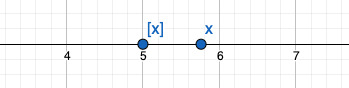
\includegraphics[width=5cm]{parte-intera.png}
    \caption{Parte intera di x}
    \label{fig:my_label}
\end{wrapfigure}
Possiamo spiegarlo in maniera semplice che è il primo numero intero che troviamo alla sinistra di x.
\begin{example}
    $[\frac{25}{10}] = 2$ \hspace{.5cm} $[-\frac{25}{10}] = -2$\\ \\
\end{example}

\vspace{-20pt}
\subsubsection{Grafico di f(x) = [x]}
\begin{wrapfigure}[8]{l}{7cm}
    \vspace{-25pt}
    \centering
    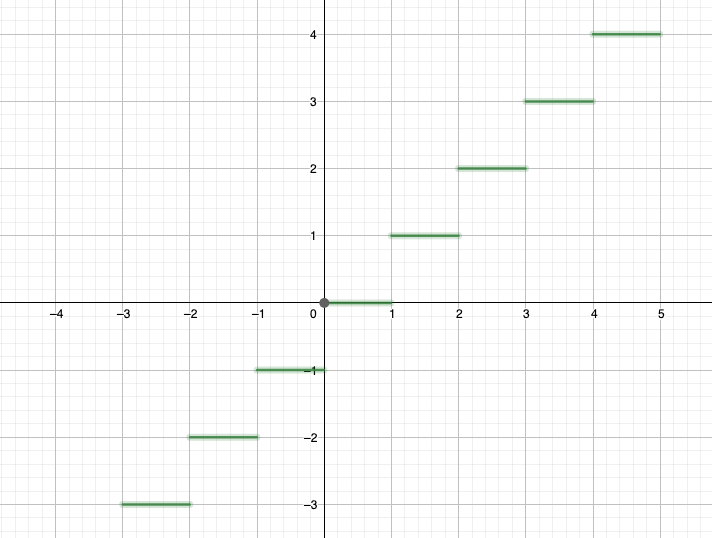
\includegraphics[width=5cm]{funzione-parte-intera.png}
    \caption{Grafico f(x) = [x]}
    \label{fig:funzione-parte-intera}
\end{wrapfigure}
\vspace{20pt}
Possiamo vedere nell'immagine [\ref{fig:funzione-parte-intera}] che tutti numeri vanno a valere in y come il valore del primo intero a sinistra.
\begin{example}
    Esempio per f(x) = [x]:\\
    $f(\frac{1}{2}) = 0$ \hspace{.3cm} $f(\frac{3}{2}) = 1$\\ \\
    $f(\frac{10}{3}) = 3$ \hspace{.3cm} $f(\frac{4}{3}) = 1$\\ \\ \\
\end{example}

\subsection{Limiti, massimi e minimi su funzioni}
Andiamo a fare una serie di definizioni prendendo due insiemi A, B tale che $A \subseteq \mathbb{R}$ e $B \subseteq \mathbb{R}$ ed una funzione $f(A)$ definita come $f: A \longrightarrow B$.
\begin{definition}[Limitata superiormente, inferiormente]
    $f$ si dice limitata superiormente se $f(A)$ è limitata superiormente. Viceversa $f$ si dice limitata inferiormente se $f(A)$ è limitata inferiormente. Se $f$ è sia limitata superiormente che inferiormente si dice che $f$ è limitata.
\end{definition}
\begin{definition}[Massimo e minimo]
    $f$ ha massimo se la sua immagine $f(A)$ ha massimo. Si dice che $M$ è il massimo di $f$ e si scrive $M = max(f)$ se $M = max(f(A))$. Ugualmente $f$ ha minimo se la sua immagine $f(A)$ ha minimo. Si dice che $m$ è il minimo di $f$ e si scrive $m = min(f)$ se $m = min(f(A))$.
\end{definition}
\begin{definition}
    Se f non è limitata superiormente e si scrive $sup(f) = +\infty$. Ugualmente se f non è limitata inferiormente, e si scrive $inf(f) = -\infty$.
\end{definition}
\begin{note}
    Rircoda che sup($f$) corrisponde a scrivere sup($f(A)$) e ugualmente inf($f$) è uguale a inf($f(A)$).
\end{note}
\begin{definition}[Punti di massimo e minimo]
    Se $f$ ha massimo allora ogni $x_0 \in A$ tale che $f(x_0) = max(f)$ si dice punto di massimo per $f$. Similmente se $f$ ha minimo allora ogni $x_0 \in A$ tale che $f(x_0) = min(f)$ si dice punto di minimo per $f$.
\end{definition}
\begin{observation}
    Il massimo di $f$ è unico mentre i punti di massimo possono essere molti.
\end{observation}

\begin{example}
    $f: \mathbb{R} \longrightarrow \mathbb{R}$ \hspace{.3cm} $f(x) = \sin{x}$ [\ref{fig:massimo_sinx}]
\end{example}
max(f) = 1 \hspace{.3cm} $x_0 = \frac{\pi}{2} + 2k\pi, k \in \mathbb{Z}$\\
\begin{wrapfigure}[4]{r}{8cm}
    \vspace{-45pt}
    \centering
    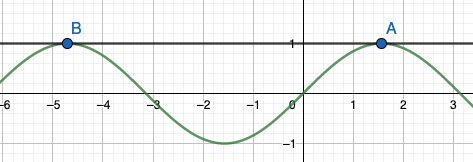
\includegraphics[width=6.5cm]{images/massimo_es1.png}
    \caption{funzione $f(x) = \sin{x}$}
    \label{fig:massimo_sinx}
\end{wrapfigure}
In questo caso essendo la funzione periodica in ogni intervallo di $x_0 = \frac{\pi}{2} + 2k\pi, k \in \mathbb{Z}$ esisterà un punto di massimo mentre il massimo rimarrà sempre 1.
\newpage
\begin{example}
    $f:(0, +\infty) \longrightarrow \mathbb{R}$ \hspace{.3cm} $f(x) = \frac{1}{x}$ [\ref{fig:massimo-minimo-frazione}]
\end{example}
In questa casistica $f$ non ha ne massimo ne minimo. Questo lo possiamo dimostrare andando ad immaginare una casistica dove esiste un massimo ed un minimo e facendo poi alcune considerazione. \\
\begin{wrapfigure}{r}{6cm}
    \vspace{-15pt}
    \centering
    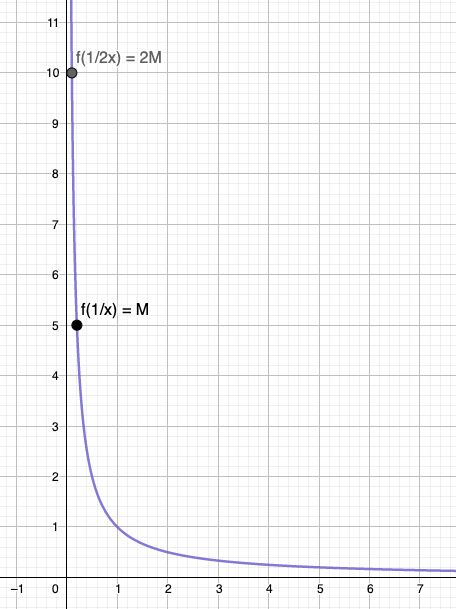
\includegraphics[width=4.5cm]{images/massimo_es2.png}
    \caption{funzione $f(x) = \frac{1}{x}$}
    \label{fig:massimo-minimo-frazione}
\end{wrapfigure}
Innanzitutto prendiamo per assurdo che $f$ avesse massimo allora $\Longrightarrow \: \: \exists \: \: m$ tale che $f(x) \leq m \: \: \forall \: \: x \in (0, +\infty)$. \\ Se in questa casistica prendessimo un punto x e dicessima che quello è il massimo, $f(\frac{1}{x}) = m$, ma se poi prendiamo un punto che è $\frac{x}{2}$ esso apparitene sempre alla funzione e $f(\frac{x}{2}) = 2m$ e $2m > m$. Quindi vediamo come non è possibile determinare un massimo.\\ \\
Questa funzione non può nemmeno avere un minimo perché $f(x) > 0 \: \: \forall \: \: x$, quindi $inf(f) = 0$. Se $f$ avesse minimo dovrebbe essere $m(f) = inf(f) = 0$ ma questo presuppone che debba esiste un $x_0$ tale che $f(x_0) = 0$ cioè $\frac{1}{x_0} = 0$, ma questo è impossibile.\\
\begin{observation}
    Consideriamo un insieme A $\subset \mathbb{R}$ e una funzione $f: A \longrightarrow \mathbb{R}$, valgono per essi le seguenti osservazioni:
    \begin{itemize}
        \item Se A ha massimo e $f$ è debolmente crescente allora $f$ ha max e max($f$) = $f$(max(A)).
        \item Se A ha minimo e $f$ è debolmente crescente allora $f$ ha min e min($f$) = $f$(min(A)).
        \item Se A ha minimo e $f$ è debolmente crescente allora $f$ ha min e min($f$) = $f$(max(A)).
        \item Se A ha massimo e $f$ è debolmente crescente allora $f$ ha max e max($f$) = $f$(min(A)).
    \end{itemize}
\end{observation}
\begin{figure}[h!]
    \begin{subfigure}{.5\textwidth}
        \centering
        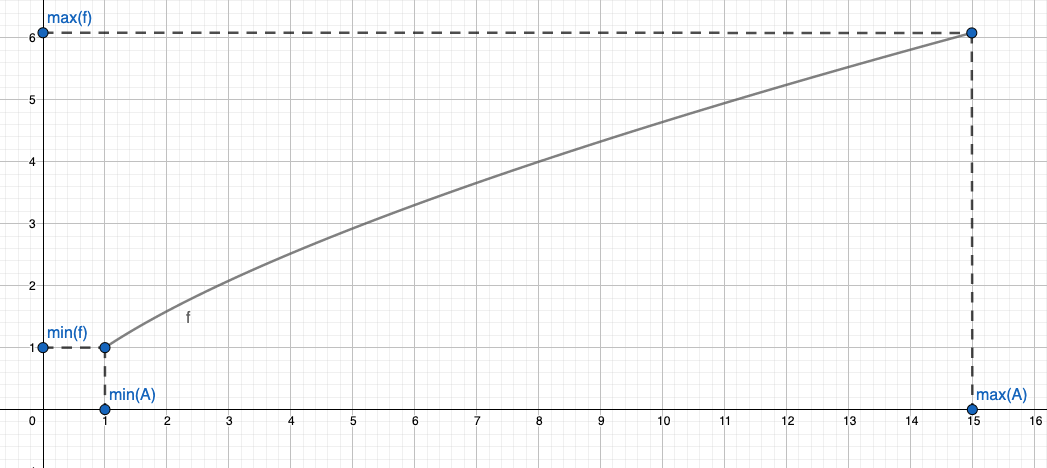
\includegraphics[width=6cm]{images/crescente-max-min.png}
        \caption{Punti max e min $f$ crescente}
        \label{fig:my_label}
    \end{subfigure}
    \begin{subfigure}{.5\textwidth}
        \centering
        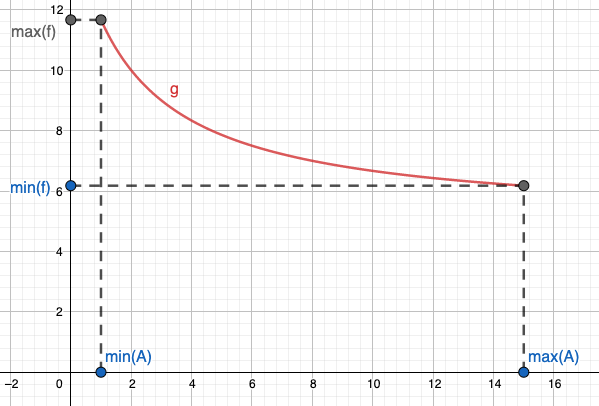
\includegraphics[width=4cm]{images/descrescente-max-min.png}
        \caption{Punti max min $f$ decrescente}
        \label{fig:my_label}
    \end{subfigure}
\end{figure}
\begin{observation}
    Se $f: A \longrightarrow \mathbb{R}$ allora m = sup($f$) se e solo se valgono queste due condizioni:
    \begin{enumerate}
        \item $f(x) \leq m \: \: \forall \: \: x \in A$ \hspace{.3cm} Questo vuol dire che m deve essere maggiore o uguale di qualsiasi f(x)
        \item $\forall \: \: \epsilon > 0 \: \: \exists \: \:  \overline{x} \in A \: \: | \: \: f(\overline{x}) > m - \epsilon$ \hspace{.3cm} Questo vuol dire che per qualsiasi valore $\epsilon$ maggiore di 0 deve esistere un $\overline{x}$ appartenendo all'insieme A tale che, se sottraiamo il valore $\epsilon$ a m il risultato deve essere inferiore a $f(\overline{x})$ ciò vuol dire che non ci sono altri valori per il quale la funzione è sempre sotto.
    \end{enumerate}
\end{observation}
